\section{Test of the Baseline Algorithm}
The baseline algorithm is now tested, using both the COV-DL algorithm and the M-SBL algorithm. In order to evaluate the performance tests are conducted on several simulated AR data sets with different specification. The aim is to see how the relationship between $N$ and $M$ affect the performance, in other word how robust the algorithm is towards low density measurements. 
The baseline algorithm is on an AR data specified by $M=8$, $L=1000$, $k=N$ and N in the range $N = [M+1, 36]$, as such $k<\frac{M(M+1)}{2}$ are withhold insuring a solution.
For each value of $N$ 5 different data sets are simulated and solved and the average MSE are used as the result. The result are plotted in figure \ref{fig:varyN1}, the MSE is plotted for both $\textbf{X}$ and $\textbf{A}$. 
Due to the performance of COV-DL not being as good as expected, a similar test is made where the true $\textbf{A}$ is given as input to M-SBL. These results are visualised in figure \ref{fig:varyN2}.    
%      
%\begin{figure}[H]
%    \begin{minipage}[t]{.45\textwidth}
%    	\centering
%		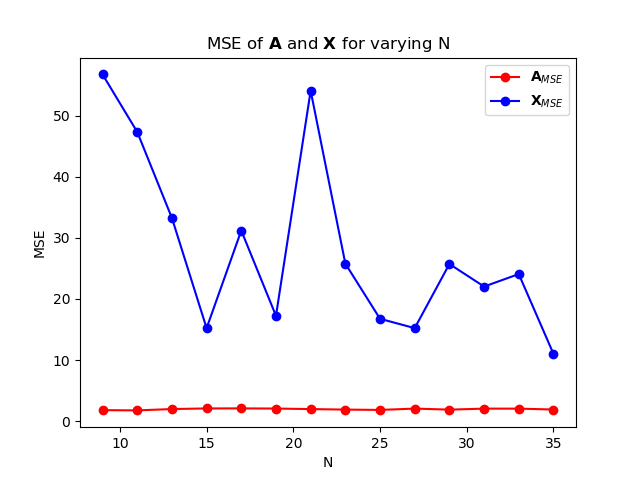
\includegraphics[scale=0.5]{figures/ch_6/varyN_recA.png}
%		\caption{ $M = 3$, $k=4$ and $L=1000$}
%		\label{fig:varyN1}
%    \end{minipage} 
%    \hfill
%    \begin{minipage}[t]{.45\textwidth}
%        \centering
%		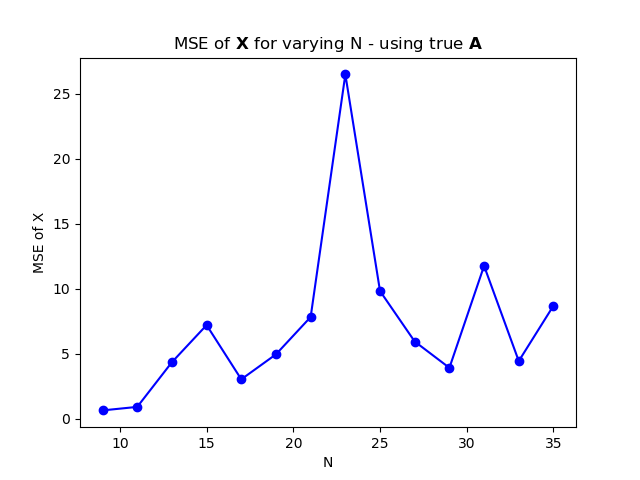
\includegraphics[scale=0.5]{figures/ch_6/varyN_trueA.png}
%		\caption{True $\textbf{A}$ $M = 3$, $k=4$ and $L=1000$ }
%		\label{fig:varyN2}
%    \end{minipage}
%\end{figure}

From the results it is seen that .. 


